\documentclass{article}
\usepackage[english,greek, main=greek]{babel}
\usepackage[utf8]{inputenc}
\usepackage{fullpage}
\usepackage{amsmath} 
\usepackage{graphicx} % for graphics and plots
\usepackage{subcaption} % for subfigures and subcaptions and \ContinuedFloat
\usepackage{placeins} % for \FloatBarrier
\usepackage{xcolor} % for colour definitions
\usepackage{listings} % for code highlighting
\usepackage{verbatim} % for file input
\usepackage{hyperref} % clickable links
\usepackage[explicit]{titlesec} % number after section name
\titleformat{\section}  % avoid numbering the table of contents
  {\normalfont\Large\bfseries}
  {}
  {0em}
  {\ifnum\value{section}=0\relax #1\else #1\ \thesection\fi}

\newcommand{\eng}[1]{\foreignlanguage{english}{#1}} % shortcut for inserting english into greek text

\useshorthands{;}
\defineshorthand{;}{?} % greek question mark instead of english semicolon

\definecolor{mGreen}{rgb}{0,0.6,0}
\definecolor{mGray}{rgb}{0.5,0.5,0.5}
\definecolor{mPurple}{rgb}{0.58,0,0.82}
\definecolor{light-gray}{gray}{0.95}
\definecolor{backgroundColour}{rgb}{0.95,0.95,0.92}

\lstdefinestyle{CStyle}{
    backgroundcolor=\color{backgroundColour},   
    commentstyle=\color{mGreen},
    keywordstyle=\color{magenta},
    numberstyle=\tiny\color{mGray},
    stringstyle=\color{mPurple},
    basicstyle=\footnotesize,
    breakatwhitespace=false,         
    breaklines=true,                 
    keepspaces=true,                 
    numbers=left,                    
    numbersep=5pt,                  
    showspaces=false,                
    showstringspaces=false,
    showtabs=false,                  
    tabsize=2,
    language=C
}

\title{
    \includegraphics[width=\textwidth]{~/Pictures/emp.png} \\
    \vskip 5cm
    Σχεδιασμός Ενσωματωμένων Συστήματων \\
    \large Άσκηση 3η
    \vskip 5cm
}

\author{
    Αναστάσιος Στέφανος Αναγνώστου \\ \large 03119051 \and
    Σαββίνα Νάστου \\ \large 03119146
}

\begin{document}

\maketitle \clearpage \tableofcontents \clearpage

\section*{Άσκηση 1}

\subsection*{Εκτίμηση Επίδοσης}

\begin{figure}[ht]
    \centering
    \begin{subfigure}{0.8\textwidth}
        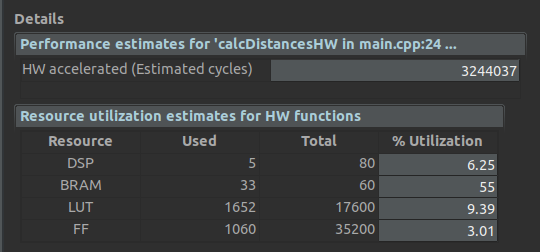
\includegraphics[width=\textwidth]{../photos/initial/cycles.png}
        \caption{Εκτίμηση \eng{hardware} κύκλων}
    \end{subfigure}
    \begin{subfigure}{0.8\textwidth}
        \includegraphics[width=\textwidth]{../photos/initial/loops.png}
        \caption{Ανάλυση βρόγχων}
    \end{subfigure}
\end{figure}

\subsection*{Πραγματική Επίδοση}

\begin{figure}[ht]
    \centering
    \includegraphics[width=0.8\textwidth]{../photos/initial/results.png}
    \caption{Πραγματικοί Κύκλοι}
\end{figure}

\subsection*{Επιτάχυνση μέσω \eng{HLS Directives}}

\begin{figure}
   \centering
   \begin{subfigure}{0.6\textwidth}
       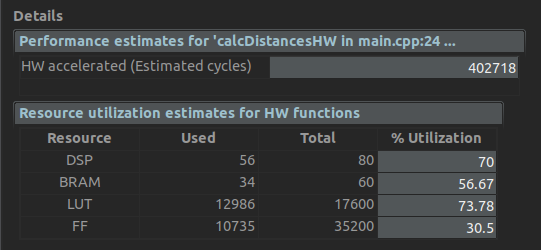
\includegraphics[width=\textwidth]{../photos/fast/cycles.png} 
        \caption{Εκτίμηση \eng{hardware} κύκλων}
   \end{subfigure}
   \begin{subfigure}{0.6\textwidth}
       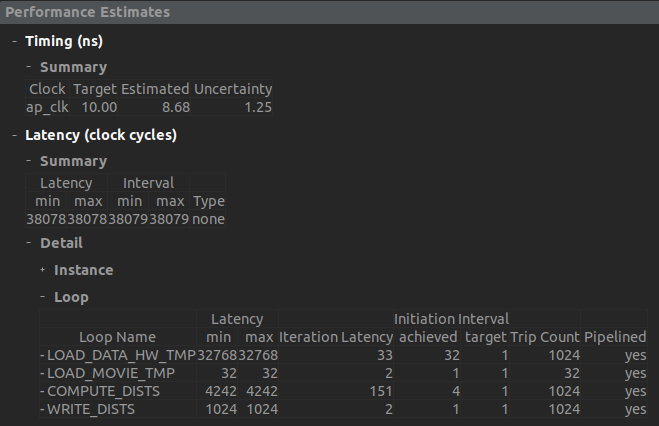
\includegraphics[width=\textwidth]{../photos/fast/loops.png} 
        \caption{Ανάλυση βρόγχων}
   \end{subfigure}
   \begin{subfigure}{0.6\textwidth}
       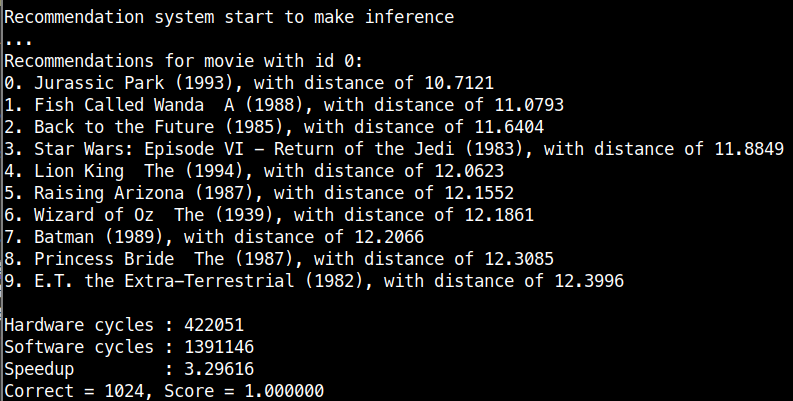
\includegraphics[width=\textwidth]{../photos/fast/results.png} 
       \caption{Πραγματικοί κύκλοι}
   \end{subfigure}
\end{figure}

\clearpage
\section*{Άσκηση 2}

Επιλέχθηκαν $INT\_BITS = 10 \text{\eng{bits}}, \text{ και } DEC\_BITS = 2
\text{\eng{bits}}$.

\begin{figure}[ht]
   \centering
   \begin{subfigure}{0.6\textwidth}
       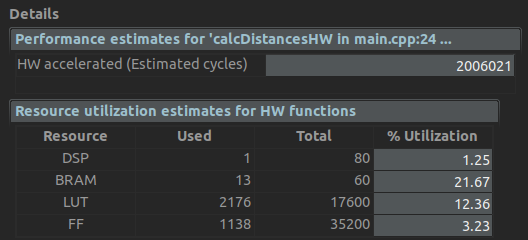
\includegraphics[width=\textwidth]{../photos/custom/cycles.png} 
        \caption{Εκτίμηση \eng{hardware} κύκλων}
   \end{subfigure}
   \begin{subfigure}{0.6\textwidth}
       \includegraphics[width=\textwidth]{../photos/custom/loops.png} 
        \caption{Ανάλυση βρόγχων}
   \end{subfigure}
\end{figure}

\begin{figure}[ht]
   \centering
   \begin{subfigure}{0.6\textwidth}
       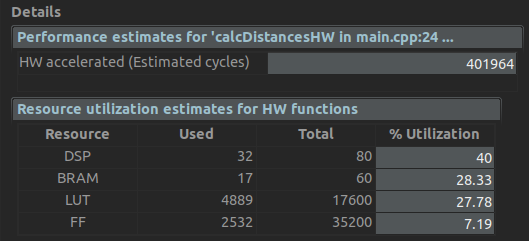
\includegraphics[width=\textwidth]{../photos/custom-fast/cycles.png} 
        \caption{Εκτίμηση \eng{hardware} κύκλων}
   \end{subfigure}
   \begin{subfigure}{0.6\textwidth}
       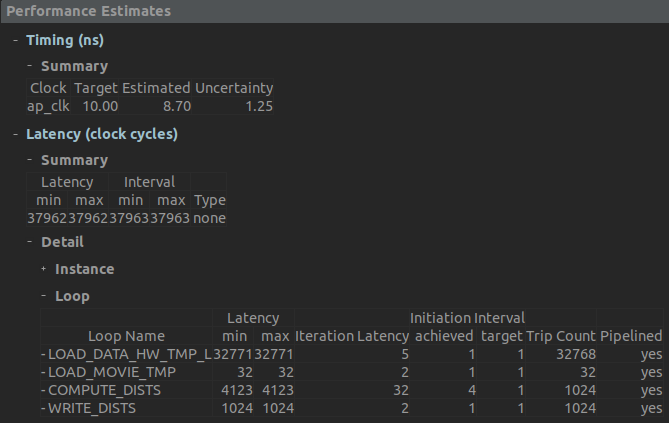
\includegraphics[width=\textwidth]{../photos/custom-fast/loops.png} 
        \caption{Ανάλυση βρόγχων}
   \end{subfigure}
   \begin{subfigure}{0.6\textwidth}
       \includegraphics[width=\textwidth]{../photos/custom-fast/results.png} 
       \caption{Πραγματικοί κύκλοι}
   \end{subfigure}
\end{figure}

\clearpage
\section*{Άσκηση 3}

\begin{figure}[ht]
   \centering
   \begin{subfigure}{0.6\textwidth}
       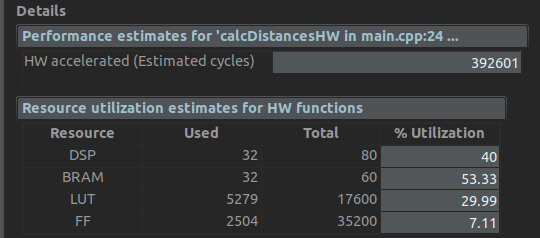
\includegraphics[width=\textwidth]{../photos/final/cycles.png} 
        \caption{Εκτίμηση \eng{hardware} κύκλων}
   \end{subfigure}
   \begin{subfigure}{0.6\textwidth}
       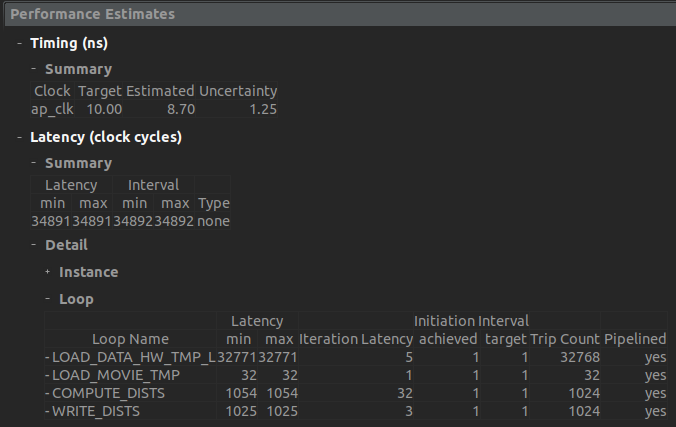
\includegraphics[width=\textwidth]{../photos/final/loops.png} 
        \caption{Ανάλυση βρόγχων}
   \end{subfigure}
   \begin{subfigure}{0.6\textwidth}
       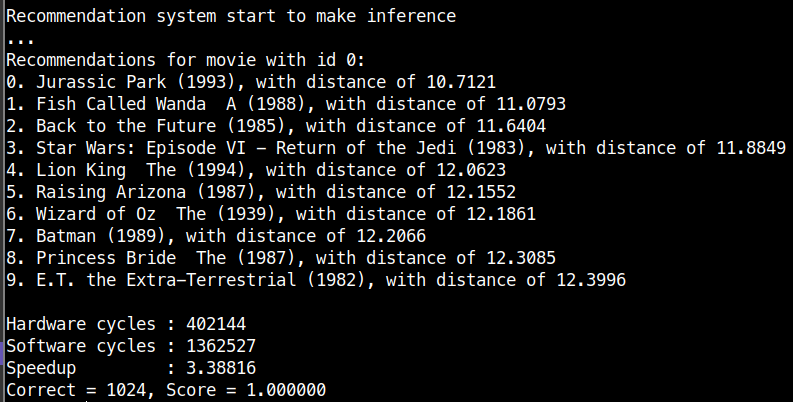
\includegraphics[width=\textwidth]{../photos/final/results.png} 
       \caption{Πραγματικοί κύκλοι}
   \end{subfigure}
\end{figure}

\end{document}

